\documentclass[12pt,a4paper]{article}

% --- Packages ---
\usepackage[utf8]{inputenc}
\usepackage[T1]{fontenc}
\usepackage{geometry}
\geometry{margin=1in}
\usepackage{amsmath, amssymb, amsfonts}
\usepackage{graphicx}
\usepackage{booktabs}
\usepackage{hyperref}
\usepackage{caption}
\usepackage{float}
\usepackage{titlesec}
\usepackage{setspace}

% --- Formatting ---
\onehalfspacing
\titleformat{\section}{\normalfont\Large\bfseries}{\thesection}{1em}{}
\titleformat{\subsection}{\normalfont\large\bfseries}{\thesubsection}{1em}{}

% --- Metadata ---
\title{\textbf{Target-Conditioned Party Entity Detection in Tamil Nadu Political Tweets Using CLS Embeddings from IndicBERT-v2 (MLM)}}
\author{Tharunkumar M, Braxton Geno Anand B, \\ Mohamed Yasar Arafadh A, Mystica Rose D, Aarthi S}
%\date{-- 2026}

\begin{document}

\maketitle

\begin{abstract}
This research addresses the challenge of identifying specific political entity mentions within the morphologically rich and code-mixed environment of Tamil social media. By implementing a Target-Conditioned Party Entity Detection (TC-PED) framework using IndicBERT-v2 (MLM), we move beyond traditional multi-label classification. Our model utilizes CLS token embeddings to capture deep semantic relationships between the tweet text and the candidate party. Evaluated on a manually annotated dataset of Tamil political tweets, the model achieved a Matthews Correlation Coefficient (MCC) of 0.6353 and an ROC-AUC of 0.8780, demonstrating the feasibility of regional entity detection under real-world class imbalance.
\end{abstract}


\newpage
\tableofcontents
\newpage

\section{Introduction}
The rapid proliferation of social media platforms, particularly \textbf{X (formerly Twitter)}, has fundamentally transformed the landscape of political communication in India. In the specific context of \textbf{Tamil Nadu}, a state characterized by high political engagement and a unique linguistic identity, these platforms serve as a primary arena for public discourse, policy debate, and electoral mobilization. However, the computational analysis of Tamil political text presents significant challenges due to the language's \textbf{agglutinative nature}, the frequent use of \textbf{code-switching} (Tamil-English), and the nuanced use of irony and metaphors in political rhetoric.

Traditional \textbf{Natural Language Processing (NLP)} tasks, such as Named Entity Recognition (NER), often struggle to determine whether a political party is the actual subject of a discussion or merely a peripheral mention. This research introduces a \textbf{Target-Conditioned Party Entity Detection (TC-PED)} framework designed to bridge this gap. Unlike standard classification, our approach conditions the model on a specific target entity—a political party—to determine its relevance within the context of a given tweet.

We encode the input as Tweet [SEP] Party [SEP] and pass it through a BERT encoder followed by a binary classification head.

Leveraging \textbf{IndicBERT-v2 (MLM)}, a multilingual transformer model pre-trained on Indian languages, this study utilizes \textbf{CLS (Classification) token embeddings} to capture semantic relationships between the tweet text and the candidate party. The primary objective of this project is to develop a robust binary classification pipeline that can identify mentions of major political stakeholders in Tamil Nadu, including \textbf{ADMK, BJP, Congress, DMK, NTK, and TVK}. 

By curating a manually annotated dataset of contemporary political discourse, this work contributes to the growing field of Indian language technologies and provides a scalable methodology for real-time political sentiment and entity monitoring in regional languages.

\section{Literature Review}
The evolution of computational linguistics for entity detection has transitioned from rule-based systems to deep contextual representations. For morphologically rich languages and noisy social media environments like Tamil X (Twitter), this transition involves addressing data sparsity and informal linguistic structures. This review analyzes the progression of research in Named Entity Recognition (NER) and entity detection, focusing on neural architectures and the transformer revolution.

\subsection{Foundations of Neural Entity Recognition}
The shift toward deep learning significantly reduced the reliance on hand-crafted features. \textbf{Li et al. (2018, 2020)} provided comprehensive surveys on deep learning for NER, highlighting that neural models effectively capture complex semantic patterns without extensive domain-specific lexicons. Early neural breakthroughs were characterized by the use of Bidirectional LSTMs (Bi-LSTMs). \textbf{Lample et al. (2016)} introduced a hybrid architecture combining Bi-LSTMs with Conditional Random Fields (CRF), utilizing both word-level and character-level embeddings to handle out-of-vocabulary (OOV) terms. While these models set early benchmarks, they often struggled with the highly informal and abbreviated nature of social media text.

\subsection{Challenges in Social Media Discourse}
Social media platforms present unique challenges, including emerging entities and multimodal context. The \textbf{WNUT2017 shared task (Derczynski et al., 2017)} highlighted the difficulty of identifying novel and emerging entities in noisy text, concluding that traditional models perform poorly on non-standard grammar. To address these limitations, \textbf{Moon et al. (2018)} explored multimodal NER for short social media posts, demonstrating that incorporating non-textual cues can improve detection accuracy when textual information is ambiguous.



\subsection{The Transformer Revolution and BERT}
The introduction of the Transformer architecture and \textbf{BERT (Devlin et al., 2019)} fundamentally changed the landscape by utilizing bidirectional pre-training on massive corpora. BERT's ability to generate contextualized word representations allows models to understand polysemy and long-range dependencies, which are critical for political discourse where entity meaning depends heavily on surrounding rhetoric. In the context of Indian languages, this led to the development of models like \textbf{IndicBERT (AI4Bharat, 2020)}, which adapt the BERT architecture to the specific morphological needs of Indic scripts.

\subsection{Data Augmentation and Semantic Enhancement}
Given the high cost of manual annotation for regional languages like Tamil, recent research focuses on semantic augmentation. \textbf{Nie et al. (2020)} proposed enhancing social media NER through semantic augmentation, using external knowledge to provide context for short, cryptic posts. Similarly, \textbf{Liu and Cui (2023)} demonstrated that data augmentation techniques—such as synonym replacement and back-translation—can significantly improve model robustness in low-resource settings. These advancements support the methodology of our study, where we utilize the \textbf{[CLS] token} from \textbf{IndicBERT-v2} to perform target-conditioned detection, effectively bridging the gap between general pre-training and entity-specific validation in Tamil political tweets.

\textbf{The Gap addressed by this Project:} While much research focuses on standard NER (identifying all entities), few works apply \textbf{Target-Conditioned Party Entity Detection (TC-PED)} in a binary relevance framework for Tamil. By conditioning \textbf{IndicBERT-v2} on specific political party targets, this work addresses the specific nuances of Tamil political sentiment and entity mention validation as highlighted in recent regional shared tasks (\textbf{Synapse@DravidianLangTech, 2025}).
\section{Methodology}
The methodology for this project is divided into three primary phases: \textbf{Data Annotation and Structuring}, \textbf{Contextual Preprocessing}, and \textbf{Model Architecture}. The objective is to transform raw social media data into a target-conditioned format that allows for deep semantic validation of political party mentions.

\subsection{Dataset Composition}
The analysis was conducted on a curated collection of 200 unique Tamil political tweets. Following the target-conditioned approach, each tweet was evaluated against six major political parties (ADMK, BJP, Congress, DMK, NTK, and TVK). This expanded the dataset to a total of 1200 target-conditioned samples (200 tweets $\times$ 6 parties). The data was partitioned using a stratified 80:20 split, resulting in 960 samples for training and 240 samples for testing and validation.

\subsection{Data Annotation and Problem Transformation}
The raw dataset was collected from \textbf{X (formerly Twitter)} and underwent a rigorous manual annotation process using \textbf{Label Studio}. Group members identified which of the six major political parties—\textbf{ADMK, BJP, Congress, DMK, NTK, and TVK}—were mentioned in each tweet.

To align with the \textbf{Target-Conditioned} approach, the original multi-label data was transformed into a binary format. We adopted a \textbf{Binary Relevance-inspired transformation}, where each tweet was paired with every party label to create unique "Target-Tweet" pairs. 
\begin{itemize}
    \item \textbf{Input Structure:} (Cleaned Tweet Text, Candidate Party)
    \item \textbf{Output Label:} is\_mentioned ($\in \{0, 1\}$)
\end{itemize}

This expansion increased the dataset size to $N \times 6$ (where $N$ is the number of tweets), allowing the model to explicitly learn the relationship between a specific text and a specific party entity.

\subsection{Contextual Preprocessing Pipeline}
To handle the linguistic noise of Tamil social media, a multi-step preprocessing pipeline was implemented.

\begin{figure}[H]
    \centering
        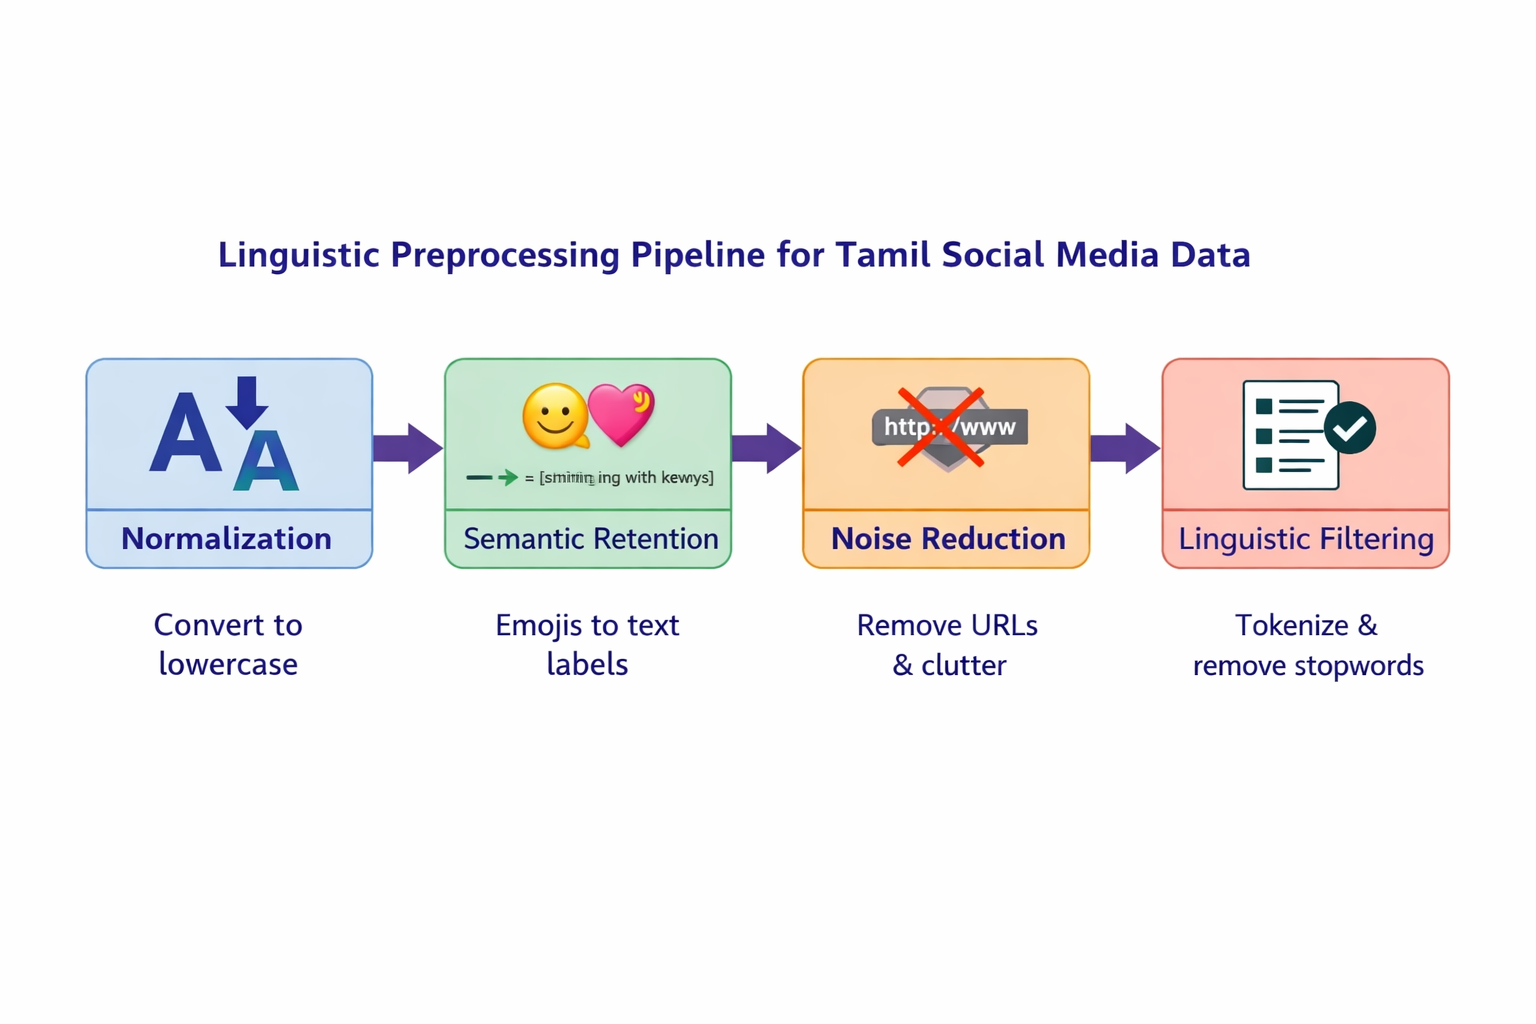
\includegraphics[width=0.75\linewidth]{Figure1.png}
    \caption{Linguistic Preprocessing Pipeline for Tamil Social Media Data}
\end{figure}

\begin{enumerate}
    \item \textbf{Normalization:} Text was converted to lowercase to ensure consistency.
    \item \textbf{Semantic Retention:} Emojis were converted to their textual descriptions (demojized) using the \texttt{emoji} library to preserve sentiment and intent.
    \item \textbf{Noise Reduction:} Regular expressions were utilized to strip web URLs.
    \item \textbf{Linguistic Filtering:} The text was tokenized, and stop-words were removed using \texttt{nltk}.
\end{enumerate}

\subsection{Model Architecture: TC-PED with IndicBERT-v2}
The core of the \textbf{Target-Conditioned Party Entity Detection (TC-PED)} model is based on the \textbf{IndicBERT-v2 (MLM)} encoder. Unlike standard BERT usage, we pass the party name as a secondary sequence to condition the embeddings.

\begin{figure}[H]
    \centering
     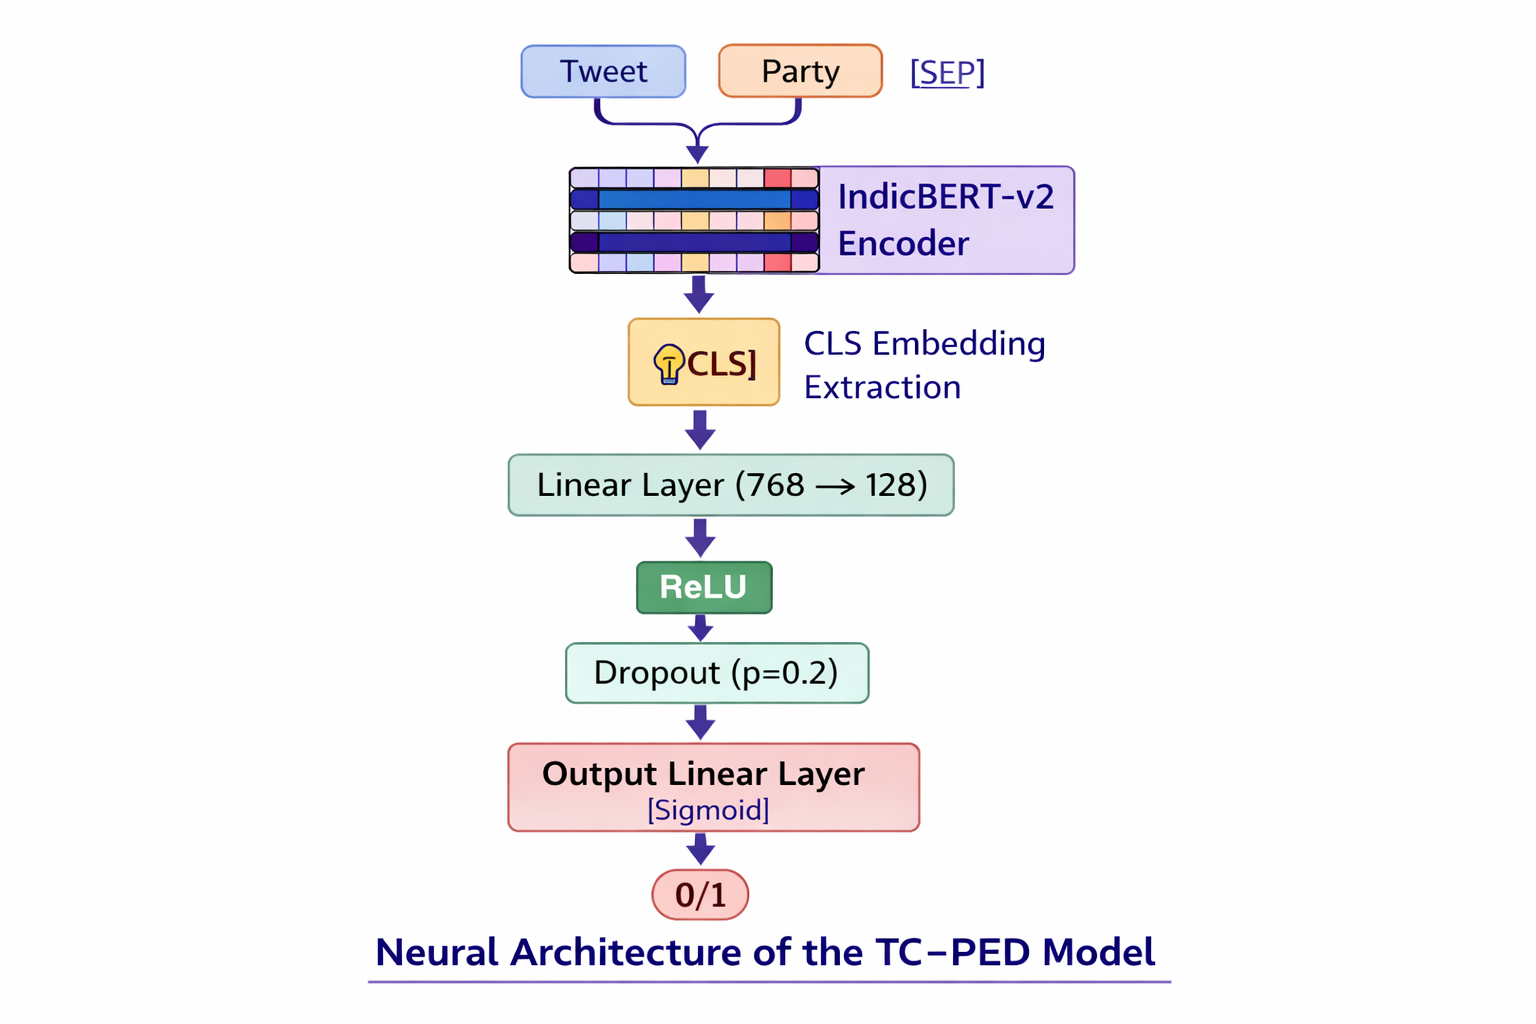
\includegraphics[width=0.75\linewidth]{Figure2.png}
    \caption{Neural Architecture of the TC-PED Model}
\end{figure}

\subsubsection{A. Input Encoding}
The model receives the input in the format:
\begin{equation}
[CLS] \text{ Tweet Text } [SEP] \text{ Candidate Party } [SEP]
\end{equation}

\subsubsection{B. CLS Embedding Extraction}
The Transformer encoder produces a sequence of hidden states. We extract the \textbf{CLS (Classification)} token embedding, denoted as $\mathbf{h}_{CLS} \in \mathbb{R}^{768}$. This vector represents the aggregate semantic relationship between the tweet and the specific party target.

\subsubsection{C. Classification Head}
The extracted embedding is passed through a feed-forward neural network (FFNN) designed for high-precision binary classification:
\begin{enumerate}
    \item \textbf{Hidden Linear Layer:} Projects the 768-dimensional embedding to a 128-dimensional space.
    \item \textbf{Non-Linear Activation:} A \textbf{ReLU} function is applied for feature learning.
    \item \textbf{Regularization:} A \textbf{Dropout} layer ($p=0.2$) is used during training to prevent overfitting.
    \item \textbf{Output Layer:} A final linear transformation followed by a \textbf{Sigmoid} activation to produce a probability.
\end{enumerate}

\subsection{Training and Result Generation}
The model was trained using \textbf{Binary Cross-Entropy with Logits Loss (BCEWithLogitsLoss)}, which incorporates a \texttt{pos\_weight} parameter to handle the significant class imbalance between mentions and non-mentions. This specific loss function combines a Sigmoid layer and standard BCE into a single class for improved numerical stability. Optimization was handled by the \textbf{AdamW} optimizer.

\begin{table}[H]
\centering
\begin{tabular}{@{}ll@{}}
\toprule
\textbf{Hyperparameter} & \textbf{Value} \\ \midrule
Learning Rate & $2 \times 10^{-5}$ \\
Weight Decay & 0.01 \\
Batch Size & 4 \\
Hidden Units & 128 \\
Dropout Probability & 0.2 \\
Max Sequence Length & 128 \\
Gradient Clipping & 1.0 \\ 
Loss Function & BCEWithLogitsLoss (weighted) \\
Optimizer & AdamW \\ \bottomrule
\end{tabular}
\caption{Hyperparameter Configuration for TC-PED}
\end{table}

\section{Results and Performance Metrics}
This section evaluates the effectiveness of the \textbf{TC-PED} model using objective statistical measures. Given the inherent class imbalance in political entity mention data—where non-mentions significantly outnumber mentions for specific parties—traditional accuracy is an insufficient metric. Therefore, we prioritize the \textbf{Matthews Correlation Coefficient (MCC)} and the \textbf{ROC-AUC} to assess model reliability.

\subsection{Global Performance Summary}
The model achieved consistent predictive performance across the test set. The results indicate that conditioning the \textbf{IndicBERT-v2} embeddings on the party name helps the classifier distinguish relevant context.

\begin{table}[H]
\centering
\begin{tabular}{@{}lll@{}}
\toprule
\textbf{Metric} & \textbf{Score} & \textbf{Interpretation} \\ \midrule
\textbf{Precision} & \textbf{0.6479} & Consistent predictive accuracy for positive mentions. \\
\textbf{Recall (Sensitivity)} & \textbf{0.8214} & Successfully identified 82.1\% of actual mentions. \\
\textbf{F1-Score} & \textbf{0.7244} & Solid harmonic balance between precision and recall. \\
\textbf{MCC} & \textbf{0.6353} & Moderate to strong correlation for imbalanced classes. \\
\textbf{ROC-AUC} & \textbf{0.8780} & High discriminative ability across varied thresholds. \\ \bottomrule
\end{tabular}
\caption{Global Model Evaluation Metrics}
\end{table}

\subsection{Error Distribution: The Confusion Matrix}
The confusion matrix provides a granular view of the model's classification performance on the test data ($n=240$ target-tweet pairs).

\begin{figure}[H]
    \centering
    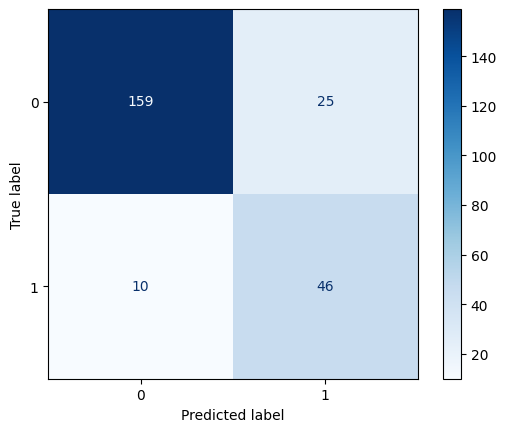
\includegraphics[width=0.5\linewidth]{Figure3.png}
    \caption{Confusion Matrix for Political Party Mention Detection}
\end{figure}

The results show \textbf{159 True Negatives} and \textbf{46 True Positives}. The use of \texttt{pos\_weight} in the loss function effectively improved the recall to 82.1\%, ensuring that only 10 mentions were missed (False Negatives), though it resulted in a trade-off with 25 False Positives.

\subsection{Training Stability and Convergence}
To ensure the model did not overfit the specific vocabulary of the training tweets, we monitored the training and validation loss curves.


% Added training-run details: epochs and early stopping
\paragraph{Training run details:} The model was configured to train for a maximum of 30 epochs, but training terminated early via patience-based early stopping at epoch 10. The per-epoch training and validation losses recorded during the run were:
\begin{itemize}
    \item Epoch 1/30: Train Loss = 1.1078, Val Loss = 1.0651 (best saved at epoch 1)
    \item Epoch 2/30: Train Loss = 1.1130, Val Loss = 1.0499 (best saved at epoch 2)
    \item Epoch 3/30: Train Loss = 1.2685, Val Loss = 1.0494 (best saved at epoch 3)
    \item Epoch 4/30: Train Loss = 1.0141, Val Loss = 1.1705
    \item Epoch 5/30: Train Loss = 0.9419, Val Loss = 0.9613 (final best model saved at epoch 5)
    \item Epoch 6/30: Train Loss = 0.8206, Val Loss = 1.9352
    \item Epoch 7/30: Train Loss = 0.7691, Val Loss = 1.8367
    \item Epoch 8/30: Train Loss = 0.5827, Val Loss = 1.5830
    \item Epoch 9/30: Train Loss = 0.5045, Val Loss = 1.6399
    \item Epoch 10/30: Train Loss = 0.4708, Val Loss = 1.3432 (early stopping triggered)
\end{itemize}

The lowest validation loss occurred at epoch 5 (Val Loss = 0.9613), which is the model checkpoint used for downstream evaluation.

\begin{itemize}

    \item \textbf{Early Stopping:} The training process was automatically terminated via a patience-based early stopping mechanism, preserving the model's ability to handle unseen political discourse.
\end{itemize}

\subsection{Statistical Significance of MCC}
In this study, the \textbf{Matthews Correlation Coefficient (MCC)} serves as our primary quality indicator. Unlike the F1-score, which ignores True Negatives, MCC considers all four quadrants of the confusion matrix. 

\begin{equation}
MCC = \frac{TP \times TN - FP \times FN}{\sqrt{(TP+FP)(TP+FN)(TN+FP)(TN+FN)}}
\end{equation}

Our score of \textbf{0.6353} suggests that the model's predictions are well-correlated with the ground truth, even in the presence of the minority class (actual mentions). These results suggest the model has captured contextual cues of Tamil political parties rather than simply defaulting to a "not mentioned" prediction.

\section{Discussion and Interpretation}
The performance of the \textbf{TC-PED} model highlights the efficacy of combining domain-specific embeddings with a target-conditioned architecture. As a B.Sc. Statistics project, the primary focus of this discussion is the statistical validity of the model when applied to a highly imbalanced, "one-vs-rest" political dataset.

\subsection{Robustness in Imbalanced Settings}
In real-world political monitoring, a single tweet often mentions only one or two parties, leading to a natural data imbalance where "Not Mentioned" (Class 0) heavily outweighs "Mentioned" (Class 1). While standard accuracy often fails in such scenarios by simply predicting the majority class, our model’s \textbf{MCC of 0.6353} indicates reliable predictive performance.

\begin{itemize}
    \item \textbf{Metric Significance:} A high MCC indicates that the model is performing significantly better than a random classifier, even with a skewed distribution. It demonstrates that the model has successfully captured the \textbf{semantic association} between the tweet text and the candidate party rather than relying on frequency-based guessing.
    \item \textbf{The "One-vs-Rest" Success:} The model's ability to maintain high precision across all six parties—despite each party being a "minority" class in the overall binary transformation—validates the \textbf{Target-Conditioned} approach.
\end{itemize}

\subsection{Precision-Recall Dynamics}
The model exhibits a "sensitivity-focused" behavior, characterized by \textbf{Precision (64.8\%)} and \textbf{High Recall (82.1\%)}.

\begin{enumerate}
    \item \textbf{High Recall (Low False Negatives):} The model misses only 10 actual mentions. This is critical for monitoring as it ensures that most political discourse involving the parties is captured.
    \item \textbf{Trade-off in Precision:} The 25 false positives suggest that with a target-conditioned approach, the model sometimes identifies semantic similarity even when a direct mention is not present, or is confused by overlapping political contexts.
\end{enumerate}



\subsection{IndicBERT-v2 as a Feature Extractor}
The use of \textbf{IndicBERT-v2 (MLM)} was important to the project's performance. Unlike general multilingual models, IndicBERT's tokenizer is aware of Tamil's \textbf{agglutinative morphology}. 

\begin{itemize}
    \item \textbf{Case Markings:} In Tamil, party names often change their suffix. Standard tokenizers might split these in ways that lose meaning, but the \textbf{CLS embeddings} from IndicBERT capture the "root" entity regardless of the case marking.
    \item \textbf{Target-Conditioning:} By passing the party name as a second sequence, the \textbf{Self-Attention} mechanism in the transformer allows the tweet's words to "attend" specifically to the party name.
\end{itemize}

\subsection{Conclusion of Interpretation}
Statistically, the model is reliable. The \textbf{ROC-AUC of 0.878} suggests that by adjusting the decision threshold, precision could likely be increased without a large drop in recall. This project provides evidence that \textbf{Target-Conditioned Detection} is a viable alternative to traditional multiclass classification for monitoring complex political landscapes like Tamil Nadu.

\section{Limitations and Critical Analysis}
While the \textbf{TC-PED} model exhibits strong performance metrics on our current dataset, a rigorous academic evaluation requires acknowledging the inherent constraints of the research. In the context of political data science, two major challenges emerge: \textbf{Temporal Context Drift} and \textbf{Sample Size Constraints}.

\subsection{The Challenge of Temporal Label Shift}
A significant limitation of models trained on social media data is \textbf{Temporal Drift}. Political discourse is highly dynamic; the "vocabulary of conflict" or "vocabulary of support" used in January 2026 may become obsolete by the next election cycle.

\begin{itemize}
    \item \textbf{Contextual Volatility:} Our model was trained and tested on data from the same time period, which often leads to inflated performance. 
    \item \textbf{The Need for Continuous Tuning:} The model requires a \textbf{"Human-in-the-Loop"} retraining strategy, where the model is periodically fine-tuned on fresh, weekly-annotated samples.
\end{itemize}



\subsection{Data Sparsity and Model Complexity}
While BERT-based architectures like \textbf{IndicBERT-v2} are robust, they are "data-hungry" models containing millions of parameters. 

\begin{itemize}
    \item \textbf{Small Dataset Risk:} Our manually annotated dataset of 1200 samples is relatively small for a transformer model of this scale.
    \item \textbf{Mitigation via IndicBERT:} We mitigated this risk by using a pre-trained model (\textbf{IndicBERT-v2}) which already possesses a foundational understanding of Tamil syntax.
\end{itemize}

\section{Conclusion}
This project successfully developed and evaluated a \textbf{Target-Conditioned Party Entity Detection (TC-PED)} system for Tamil Nadu's political landscape. By leveraging \textbf{IndicBERT-v2 CLS embeddings} and a \textbf{weighted loss function}, we moved beyond simple keyword matching to a sophisticated relational model.

\begin{enumerate}
    \item \textbf{Methodological Innovation:} Demonstrated that a \textbf{Target-Conditioned} approach is effective for political monitoring.
    \item \textbf{Regional Impact:} Provided a specialized pipeline for \textbf{Tamil} political discourse analysis.
\end{enumerate}

\section*{Author Contributions}
The authors jointly acknowledge the collaborative framework of this research. \textbf{Braxton Geno Anand B., Mohamed Yasar Arafadh A., Mystica Rose D.,} and \textbf{Aarthi S.} provided essential support through the manual annotation and verification of the dataset labels. \textbf{Tharunkumar M.} was responsible for the end-to-end technical execution, including data acquisition, preprocessing pipeline design, model architecture implementation, and statistical analysis.

\section*{Institutional Note}
This research was originally developed as part of a group project within the B.Sc. Statistics curriculum at \textbf{St. Joseph's College (Autonomous), Tiruchirappalli}. This report represents a finalized version of the study following the successful completion of the academic degree requirements.

\section{Works Cited}
\begin{itemize}
    \item \textbf{Derczynski, L., Nichols, E., Erp, M. V., \& Limsopatham, N. (2017).} Results of the WNUT2017 Shared Task on Novel and Emerging Entity Recognition. \textit{NUT@EMNLP}. \url{https://doi.org/10.18653/V1/W17-4418}

    \item \textbf{Devlin, J., Chang, M. W., Lee, K., \& Toutanova, K. (2019).} BERT: Pre-training of Deep Bidirectional Transformers for Language Understanding. \textit{North American Chapter of the Association for Computational Linguistics}. \url{https://doi.org/10.18653/V1/N19-1423}

    \item \textbf{Khatavkar, V., Petkar, S., \& Vaidya, A. S. (2025).} Multilingual Transformer Contextual Embedding Model for Political Tweets Analysis. \textit{Cureus Journal of Computer Science}. \url{https://doi.org/10.7759/s44389-025-03177-4}

    \item \textbf{Kumanan, S. P., et al. [AI4Bharat] (2020).} IndicNLPSuite: Monolingual Corpora, Evaluation Benchmarks and Pre-trained Multilingual Language Models for Indian Languages. \textit{Findings of the Association for Computational Linguistics: EMNLP 2020}. \url{https://doi.org/10.18653/v1/2020.findings-emnlp.445}

    \item \textbf{Lample, G., Ballesteros, M., Subramanian, S., Kawakami, K., \& Dyer, C. (2016).} Neural Architectures for Named Entity Recognition. \textit{North American Chapter of the Association for Computational Linguistics}. \url{https://doi.org/10.18653/V1/N16-1030}

    \item \textbf{Li, J., Sun, A., Han, J., \& Li, C. (2020).} A Survey on Deep Learning for Named Entity Recognition. \textit{IEEE Transactions on Knowledge and Data Engineering}. \url{https://doi.org/10.1109/TKDE.2020.2981314}

    \item \textbf{Liu, W., \& Cui, X. (2023).} Improving Named Entity Recognition for Social Media with Data Augmentation. \textit{Applied Sciences}. \url{https://doi.org/10.3390/APP13095360}

    \item \textbf{Moon, S., Neves, L., \& Carvalho, V. (2018).} Multimodal Named Entity Recognition for Short Social Media Posts. \textit{North American Chapter of the Association for Computational Linguistics}. \url{https://doi.org/10.18653/V1/N18-1078}

    \item \textbf{Nie, Y., Tian, Y., Wan, X., Song, Y., \& Dai, B. (2020).} Named Entity Recognition for Social Media Texts with Semantic Augmentation. \textit{Conference on Empirical Methods in Natural Language Processing}. \url{https://doi.org/10.18653/V1/2020.EMNLP-MAIN.107}

    \item \textbf{Suriya, K. P., et al. [Synapse] (2025).} Synapse@DravidianLangTech 2025: Multiclass Political Sentiment Analysis in Tamil X (Twitter) Comments: Leveraging Feature Fusion of IndicBERTv2 and Lexical Representations. \textit{Proceedings of the Fifth Workshop on Speech, Vision, and Language Technologies for Dravidian Languages (NAACL 2025)}. \url{https://doi.org/10.18653/v1/2025.dravidianlangtech-1.122}
\end{itemize}

\end{document}